\section{Choice of Parameters}
\label{Sec: Choice of Parameters}
Our HOPS/AWE algorithm is based on two smallness assumptions:
\begin{enumerate}
\item \text{Boundary Perturbation: $g(x)=\varepsilon f(x),$ $\varepsilon\in\mathbb R$, $\varepsilon \ll 1$,}
\vspace{-2mm}
\item \text{Frequency Perturbation: $\omega=(1+\delta)\underline{\omega}=\underline{\omega}+\delta\underline{\omega},$ $\omega\in\mathbb R$, $\delta \ll 1$,} 
\end{enumerate}
with the additional assumption that $f$ is sufficiently smooth ($f\in C^2$ \cite{NichollsReitich99,NichollsReitich03b} or even Lipschitz \cite{hu2005analyticity}). Numerical simulations show that our HOPS/AWE algorithm can handle larger perturbations of $\varepsilon$ (the height/slope) in comparison to $\delta$ (the frequency). With modest test parameters and a period of $d=2\pi$, we are able to perturb the value of $\varepsilon$ (to $\varepsilon=0.1$ or even $\varepsilon=0.2$) and still get reasonable convergence results. At a value around $\varepsilon = 10^{-4}$, our HOPS/AWE algorithm converges to machine precision provided that we sum to high enough Taylor orders.
\vspace{-13mm}
\begin{figure}[H]
    \centering
    \subfloat[\centering Large $\varepsilon$, Small $\delta$ ]{{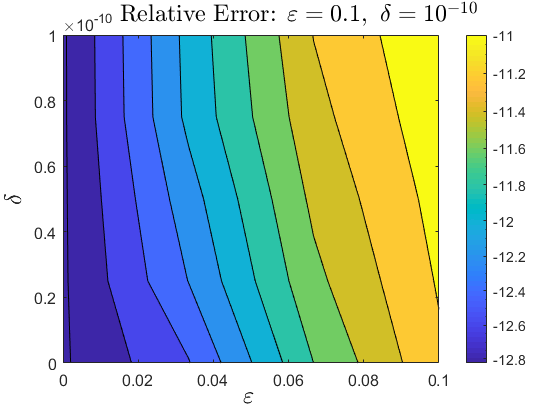
\includegraphics[width=7.6cm]{sections/7_conclusions_and_future_directions/Large_Eps_Small_Delta_2.png} }}%
    %\qquad
    \subfloat[\centering Small $\varepsilon$, Large $\delta$ ]{{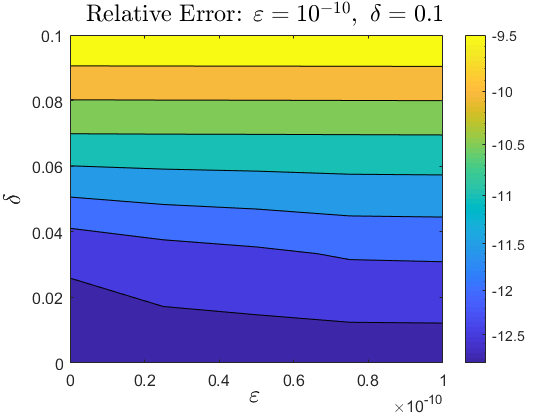
\includegraphics[width=7.6cm]{sections/7_conclusions_and_future_directions/Small_Eps_Large_Delta_2.png} }}%
    \vspace{3 mm}
    \caption{A contour plot of the relative error computed with our HOPS/AWE algorithm by holding $N=M=8$ Taylor orders fixed. In Figure $34\text{(a)}$ we expand up to $\Eps = 0.1$ and $\delta = 10^{-10}$ simultaneously with $N=M=8$ Taylor orders. In Figure $34\text{(b)}$ we expand up to $\Eps = 10^{-10}$ and $\delta = 0.1$ simultaneously with $N=M=8$ Taylor orders.}%
    \label{fig:example}%
\end{figure}
\vspace{-18mm}
Supplementary testing in both the upper and lower layers confirms that our HOPS/AWE algorithm is better suited towards larger $\varepsilon$.
%\begin{flushleft}
\newline
\\
\textbf{Predictions:} Our HOPS/AWE methodology takes advantage of exact enforcement of the \gls{owc} at an artificial boundary in order to truncate the computational domain to one of finite extent. After flattening the surface, the DNOs recover information through the solution stored at the interface. We suspect that this process mitigates large perturbations of the height/slope. By following techniques developed in \cite{NichollsReitich00b,NichollsTaber06,Nicholls16b,NichollsShen08}, we intend to rigorously prove that the TFE method is analytic when $\varepsilon$ is large. Additionally, we are interested in perturbing other physical parameters in the context of layered media problems. These are discussed in the engineering literature \cite{mashayekh2018parameter,mashayekh2018parameter2}.